% !TEX root = rebuttal.tex
\documentclass[10pt,twocolumn,letterpaper]{article}

\usepackage[rebuttal]{cvpr}
\usepackage{eccvabbrv}
\usepackage{graphicx}
\usepackage{booktabs}
\usepackage{amsfonts}
\usepackage{amsmath}
\usepackage{xcolor}
\usepackage[accsupp]{axessibility}
\usepackage{float}

\definecolor{eccvblue}{rgb}{0.12,0.49,0.85}
\usepackage[pagebackref,breaklinks,colorlinks,citecolor=eccvblue]{hyperref}

\newif\ifshowreviewtags
\showreviewtagsfalse
\newcommand{\reviewtag}[1]{\ifshowreviewtags{\textcolor{eccvblue}{\scriptsize [#1]}}\fi}
\newcommand{\reviewstatus}[1]{\ifshowreviewtags{\par\vspace{0.5mm}\noindent\parbox{\linewidth}{\raggedright\textcolor{red}{\scriptsize [Unanswered / unchecked: #1]}}\par\vspace{0.8mm}}\fi}

\def\paperID{153}
\def\confName{ECCV}
\def\confYear{2026}


\begin{document}

\title{OREO: Fidelity Alignment in 3D Generation via On-the-fly Rendering-Editing Optimization}

\maketitle
\thispagestyle{empty}
\appendix
\renewcommand{\thefigure}{R\arabic{figure}}
\renewcommand{\thetable}{R\arabic{table}}
\vspace{-5mm}

\begin{figure}[H]
\vspace{-2mm}
\centering
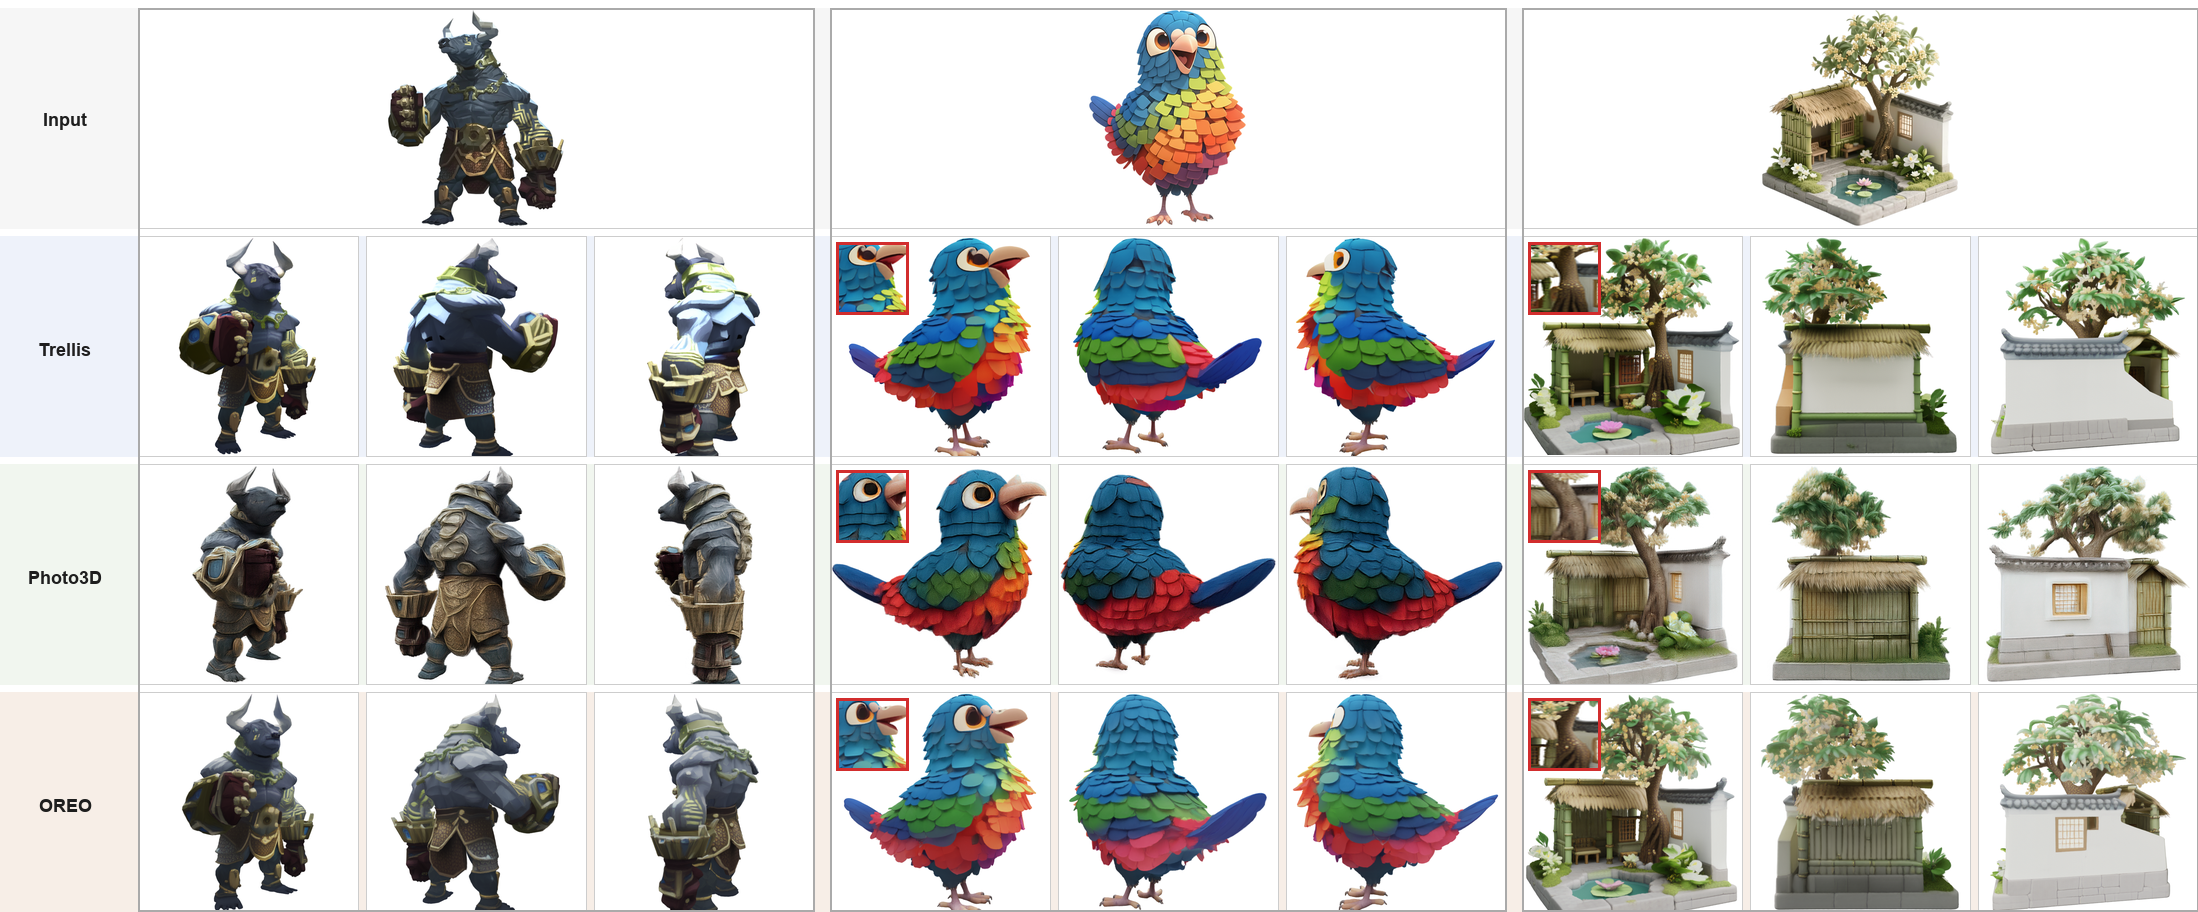
\includegraphics[width=\linewidth]{figures_rebuttal/mv_comparison_00250_04198_03360.png}
\caption{Additional multi-view qualitative comparison.}
\label{fig:mv_comparison}
\vspace{-2mm}
\end{figure}

We sincerely thank all reviewers for their constructive comments. We will revise the paper with high-resolution visualizations, expanded related work, and clearer discussions of failure cases and editing-guidance limitations.

\vspace{-2mm}
\section*{To Reviewer Nz3M}
\reviewstatus{R1-Min2}

\noindent{\em\textbf{Q1. Evaluation on other dataset.}} \reviewtag{R1-Maj1, R1-Sug1}
Thanks for the suggestion. The proposed Objaverse is Trellis's training set, so we instead evaluate on Toy4K, which is Trellis's official test set. Results are in Table~\ref{tab:toy4k}. While OREO targets generalization on concept-rich input images, it still improves over baselines on standard benchmarks.

\noindent{\em\textbf{Q2. Comparison with distillation baselines.}} \reviewtag{R1-Maj2, R1-Sug2}
Thank you for pointing this out. The proposed Magic3D and ProlificDreamer are text-to-3D, optimization-based methods, whereas we investigate image-to-3D learning-based generation. Nevertheless, we compare against DMD, a widely-used distillation loss inspired by ProlificDreamer, as an ablation in Sec.~4.3 and Fig.~5 of the main paper. It underperforms our pseudo-GT supervision on all metrics.

\noindent{\em\textbf{Q3. Human evaluation results.}} \reviewtag{R1-Maj3, R1-Sug3}
We conducted a human preference study with 20 participants evaluating all 100 test samples of the used dataset on multi-view renderings' fidelity and consistency with the input image. OREO is preferred by 41\% of responses, compared to 36\% for Photo3D and 23\% for Trellis. Full results will be in the revision.

\noindent{\em\textbf{Q4. Computational overhead.}} \reviewtag{R1-Maj4, R1-Min1, R1-Sug4}
The 9-step image editing accounts for 81\% of each training iteration if executed sequentially. We can mitigate this overhead by wrapping it as an async service and overlapping editing calls with the next-batch rollout, reducing the effective wait to 45\% on the same hardware with negligible impact on quality. We will include this in the next version.

\vspace{-2mm}
\section*{To Reviewer Ydh5}
\reviewstatus{none}

\noindent{\em\textbf{Q1. Limited qualitative results and figure readability.}} \reviewtag{R2-Maj1, R2-Maj1a, R2-Maj1b, R2-Maj1c, R2-Maj1d, R2-Maj2, R2-Min1, R3-Qual1, R3-Qual3}
Thank you for the suggestion. Fig.~\ref{fig:mv_comparison} provides additional multi-view comparisons with Trellis and Photo3D, where zoomed-in regions highlight fine-grained texture and structure details. We will add more high-resolution examples and highlighted details in the revision.

\noindent{\em\textbf{Q2. Dataset detail.}} \reviewtag{R2-Maj3, R2-Sug1}
We collect web images from mixed sources and manually filter them to ensure rich appearance details and alignment with realistic user scenarios. We will add these details in the next version and release this dataset.

\noindent{\em\textbf{Q3. Evaluation on other dataset.}} \reviewtag{R2-Maj4, R2-Sug2}
Thanks for the suggestion. Following Trellis, we evaluate on Toy4K with metrics from the official evaluation. Results are shown in Table~\ref{tab:toy4k}.

\vspace{-2mm}
\section*{To Reviewer 1rPv}
\reviewstatus{none; R3-Sug1 is covered by R3 Q1--Q4}

\begin{figure}[t]
\vspace{-2mm}
\centering
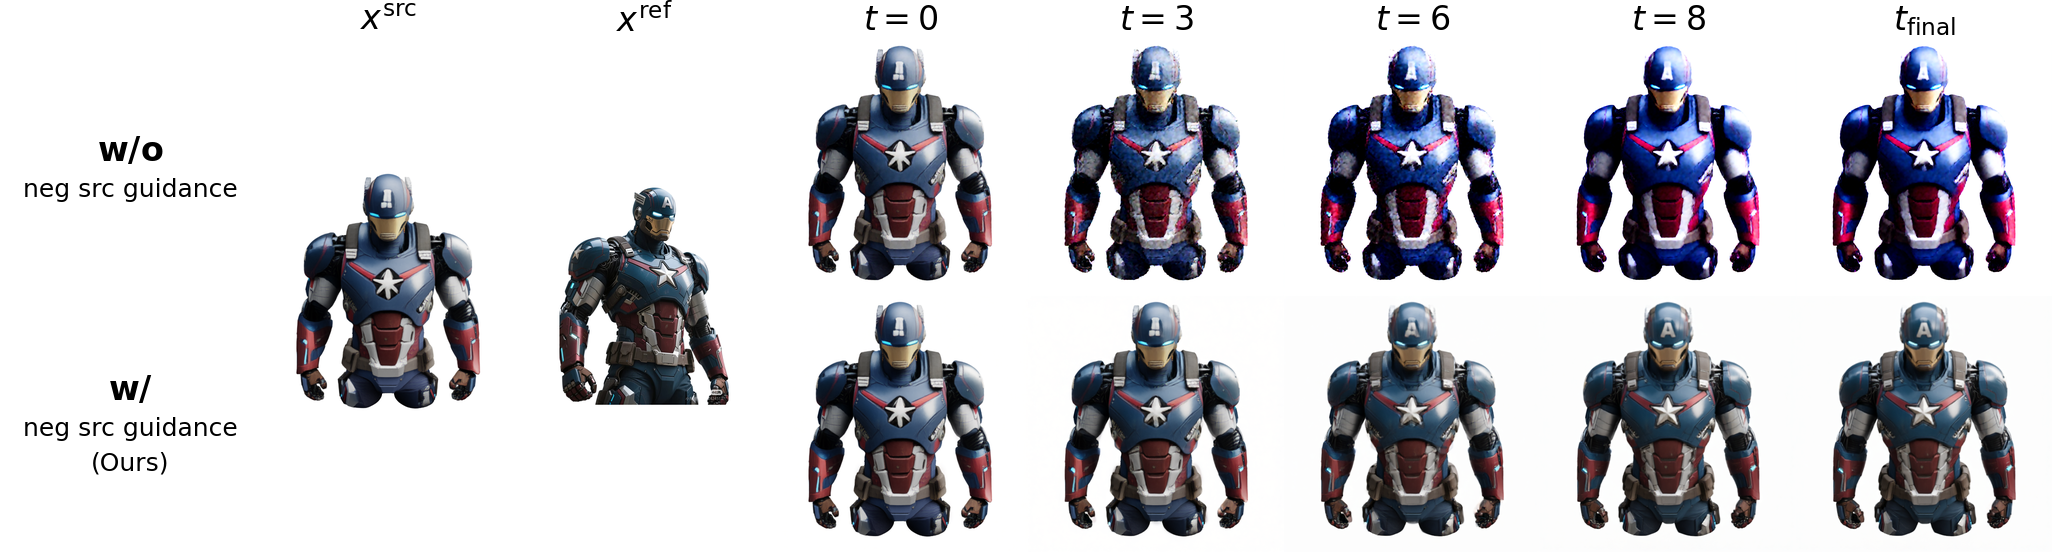
\includegraphics[width=\linewidth]{figures_rebuttal/comparison_grid.png}
\caption{Qualitative visualization of editing trajectories with/without negative source guidance in Reinforced Editing.}
\label{fig:neg_src_traj}
\end{figure}

\begin{table}[t]
\vspace{-1mm}
\centering\scriptsize
\begin{tabular}{lcccc}
\toprule
Method & CLIP$\uparrow$ & FD$_{\text{inc}}\downarrow$ & FD$_{\text{dino}}\downarrow$ & KD$_{\text{dino}}\downarrow$ \\
\midrule
Trellis & 86.78 & 9.23 & 66.82 & 0.73 \\
Photo3D & 86.89 & \textbf{9.09} & 76.98 & \textbf{0.70} \\
\midrule
OREO & \textbf{87.12} & 9.12 & \textbf{62.54} & \textbf{0.70} \\
OREO (w/o noise update) & 86.83 & 9.39 & 67.41 & 0.72 \\
\bottomrule
\end{tabular}
\caption{Evaluation on Toy4K following the Trellis protocol.}
\label{tab:toy4k}
\vspace{-3mm}
\end{table}

\noindent{\em\textbf{Q1. Limited qualitative results and figure quality.}} \reviewtag{R3-Qual1}
Thanks for the advice. In Fig.~\ref{fig:mv_comparison}, we provide additional multi-view comparisons including back views for more comprehensive angle coverage. For example, OREO better reconstructs the eye and spotted feather patterns on the parrot, and the twisted tree trunk shape in the courtyard. We will include more examples with additional angles in the next version.

\noindent{\em\textbf{Q2. Hard-to-interpret ablation results.}} \reviewtag{R3-Qual2}
The noise update strengthens alignment with the editing model's prior but may inherit its color bias on certain cases such as the golem.
But as confirmed by Table~3 in our manuscript and Table~\ref{tab:toy4k} which measure distributional similarity to ground-truth renderings, this mechanism yields consistently better aggregate metrics overall. Fig.~\ref{fig:mv_comparison} also shows more consistent back colors on the minotaur than pretrained Trellis.

\noindent{\em\textbf{Q3. Explanation of Eq.~7 is unclear.}} \reviewtag{R3-Clar1}
The negative source branch in Eq.~7 acts as an auxiliary regularizer, stabilizing reference-guided editing.
The intermediate steps in Fig.~\ref{fig:neg_src_traj} show that removing it causes color over-saturation and insufficient structural changes, e.g., the ``A'' on the helmet is missing.
We will expand Sec.~3.3 with this visualization.

\noindent{\em\textbf{Q4. Computational cost and edit prompts.}} \reviewtag{R3-Clar2, R3-Clar3, R3-Min1, R3-Min2}
Backpropagating through the differentiable renderer and decoder requires about 10GB VRAM with gradient checkpointing.
For the editing instructions for Qwen-Image-Edit and NanoBanana, we adapt the effective prompts as verified in Photo3D, and will include the exact text in the revision.

\end{document}

